\documentclass[dvipdfmx]{beamer}
\usepackage{bxdpx-beamer}% dvipdfmxなので必要
\usepackage{pxjahyper}% 日本語で'しおり'したい
%\usepackage{etex}
%\usetheme{Warsaw}
\usetheme{Malmoe}
%\usetheme{AnnArbor}
%\usetheme{Hannover}
%\usetheme{Bergen}
%\usetheme{Berlin}
%\usetheme{Singapore}
%\usetheme{Montpellier}
%\usetheme{Pittsburgh}
\usepackage{graphicx}
\usepackage{latexsym,amssymb}
%\usepackage{epsbox}
%\usepackage{multirow}
\usepackage{fancybox}
\usepackage{fancyvrb}
%\usepackage{listings}
\usepackage{tabularx}
\usepackage{tikz}
\usetikzlibrary{calc,shapes}
%\usepackage{pstricks,pst-node,pst-tree}
%\usepackage{multimedia}
%\usepackage{pstricks,pst-node,pst-tree}
%\usepackage{pst-all}
%\include{prooftree}
%\lstloadlanguages{pascal}
\renewcommand{\kanjifamilydefault}{\gtdefault}
\renewcommand{\familydefault}{\sfdefault}

%\include{cmacros}

\graphicspath{{figs261027/}}

\newcommand{\greentext}[1]{{\color[rgb]{0,0.5,0}{#1}}}
\newcommand{\redtext}[1]{{\color[rgb]{0.8,0,0}{#1}}}
\newcommand{\bluetext}[1]{{\color[rgb]{0,0,0.8}{#1}}}

\newcommand{\tuple}[1]{\langle{#1}\rangle}

\newcommand{\First}{\mathsf{First}_1}
\newcommand{\Follow}{\mathsf{Follow}_1}

%%pdt simulation

\newcommand{\pdtline}[6]{%
    \uncover<#6->{
    \node at (${#5}*(0,-.3)+(0,.3)$) {$\vdash$};%
    \node at (${#5}*(0,-.3)+(1.5,.3)$) {\parbox{12em}{(#1,}};%
    \node at (${#5}*(0,-.3)+(4.5,.3)$) {\parbox{10em}{#2,}};%
    \node at (${#5}*(0,-.3)+(5.7,.3)$) {\parbox{10em}{#3)}};%
    \node at (${#5}*(0,-.3)+(8,.3)$) {\parbox{20em}{#4}};%
    }
}

\newcommand{\initpdtline}[6]{%
    \uncover<#6->{
    \node at (${#5}*(0,-.3)+(1.5,.3)$) {\parbox{12em}{(#1,}};%
    \node at (${#5}*(0,-.3)+(4.5,.3)$) {\parbox{10em}{#2,}};%
    \node at (${#5}*(0,-.3)+(5.7,.3)$) {\parbox{10em}{#3)}};%
    \node at (${#5}*(0,-.3)+(8,.3)$) {\parbox{20em}{#4}};%
    }
}

\newtheorem{Def}{定義}
\newtheorem{Lem}{補題}
\newtheorem{Thm}{定理}
\newtheorem{Prop}{命題}

\definecolor{lightlightgrey}{rgb}{0.95,0.95,0.95}



%\newcommand{\greentext}[1]{{\color[rgb]{0,0.5,0}{#1}}}
%\newcommand{\redtext}[1]{{\color[rgb]{0.8,0,0}{#1}}}

\newcommand{\lecturedate}{2026/10/27}

\cornersize{0.25}

\setbeamertemplate{frametitle}[default][center]
\setbeamertemplate{footline}{\hfill
コンパイラ\quad\lecturedate
\hfill\insertframenumber/\inserttotalframenumber\hspace*{1zw}}
\newcounter{coffee}
\setbeamercovered{transparent=10}
\title{コンパイラ(8)}
\date{\lecturedate}
\begin{document}

\frame{\titlepage}

\section{コード最適化}

\begin{frame}
  \begin{center}
    {\Huge コード最適化}
  \end{center}
\end{frame}

\subsection{概要}

\begin{frame}
  \frametitle{コード最適化}

  実行の意味を変えることなく実行を高速化すること。

  \begin{list}{}{}
    \item 実行の意味：入力と出力\\
          最適化の対象によって入力と出力は変わる。\\
          \greentext{プログラム解析が必要}
  \end{list}


  \begin{itemize}
    \item 機械独立なコード最適化\\
          \quad =3番地コードのレベルで実行を効率化
    \item 機械依存なコード最適化\\
          \quad =対象マシンのアーキテクチャに依存\\
          \qquad (VLIW、マルチコアなど)
  \end{itemize}

\end{frame}

\subsection{局所最適化}

\begin{frame}
  \frametitle{基本ブロック}

  最後以外分岐のない文の並び

  \begin{center}
    \only<1>{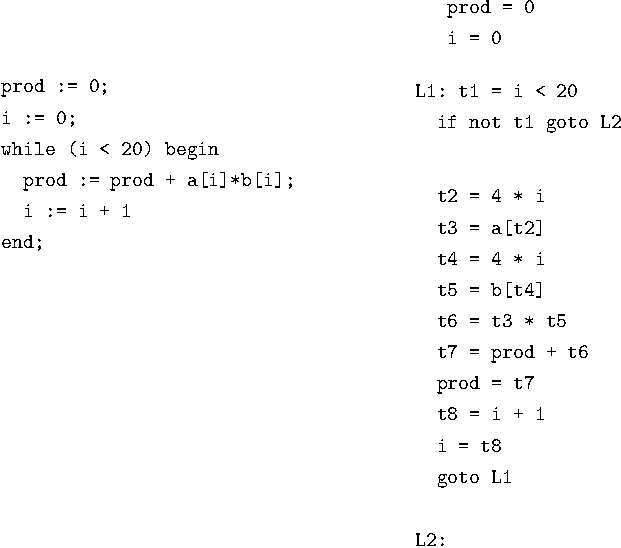
\includegraphics[width=.8\textwidth]{basic-block-fig-r2-crop.pdf}}
    \only<2>{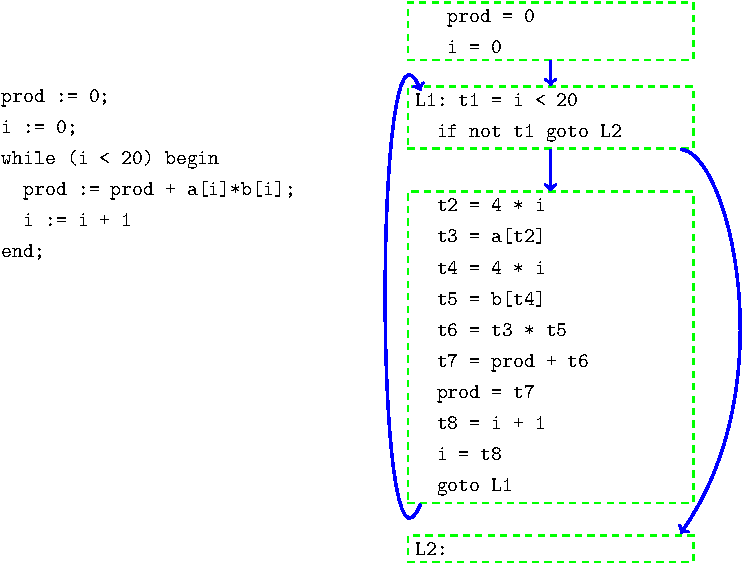
\includegraphics[width=.8\textwidth]{basic-block-fig2-r2-crop.pdf}}
  \end{center}

\end{frame}

\begin{frame}
  \frametitle{局所最適化}

  基本ブロック内だけを見て最適化すること

  覗き穴最適化(Peep-hole optimization)

  \begin{itemize}
    \item 定数伝播(constant propagation)\\
          \greentext{定数の計算、参照を定数そのものでおきかえる}
    \item 共通部分式の削除(common subexpression elimination)\\
          \greentext{共通の部分式を抽出して結果を一時変数に保存
            するようにして、二回目以降計算しない。}
    \item コピー伝播(copy propagation)\\
          \greentext{余分な変数の仲介を減らす。}\\
          \greentext{データ依存性を減らして命令の並列発行が可能
            になる場合がある。}
    \item 不要コードの除去(deadcode elimination)\\
          \greentext{使われない変数に関する計算を消去する。}
    \item 代数的性質の利用\\
          \greentext{演算子が持つ代数的性質(可換則、結合則、分
            配則、計算のためのコストなど)}
  \end{itemize}
\end{frame}

\begin{frame}
  \frametitle{DAGによる局所最適化}

  DAG=Directed Asyclic Graph\\
  \greentext{閉路(ループ)をもたない有効グラフ}

  \greentext{基本ブロック内のデータ依存性を一意的に表現}

  DAGの構成アルゴリズム 6.6


\end{frame}

\begin{frame}
  \frametitle{DAGの構成}
  \begin{tabular}{cc}
    \begin{minipage}{.45\textwidth}

      \begin{tikzpicture}
        \node[draw,circle] (a0) at (0,0) {$a_0$};
        \node[draw,circle] (b0) at (1.5,0) {$b_0$};
        \node[draw,circle] (c0) at (3,1) {$c_0$};
        \uncover<2->{\node[draw,circle] (AST) at (0.75,1) {$\ast$};}
        \uncover<2-6>{\node at ($(AST)+(0.5,0)$) {$x$};}
        \uncover<3->{\node[draw,circle] (PLUS) at (2,2) {$+$};
          \node at ($(PLUS)+(0.5,0)$) {$y$};}
        \uncover<4->{\node at ($(AST)+(0.8,0)$) {$,d$};}
        \uncover<5->{\node[draw,circle] (MIN) at (2,3.5) {$-$};
          \node at ($(MIN)+(0.5,0)$) {$e$};}
        \uncover<7->{\node[draw,circle] (PL2) at (2,5) {$+$};
          \node at ($(PL2)+(0.5,0)$) {$x$};}
        \only<2->{
          \path[-] (a0) edge (AST) (b0) edge (AST);
        }
        \only<3->{
          \path[-] (AST) edge (PLUS) (c0) edge (PLUS);
        }
        \only<5->{
          \path[-] (MIN) edge (AST) (MIN) edge (c0);
        }
        \only<7->{
          \path[-] (PL2) edge (AST) (PL2) edge (MIN);
        }
      \end{tikzpicture}

    \end{minipage}
     &
    \begin{minipage}{.4\textwidth}

      \begin{tikzpicture}
        \node[anchor=west] at (0,3) {\texttt{x=\redtext{a}*\redtext{b}}};
        \only<1,3->{\node[anchor=west] at (0,2.5) {\texttt{y=x+\redtext{c}}};}
        \only<1,4->{\node[anchor=west] at (0,2) {\texttt{d=\redtext{a}*\redtext{b}}};}
        \only<1,5->{\node[anchor=west] at (0,1.5) {\texttt{e=d-\redtext{c}}};}
        \only<1,7->{\node[anchor=west] at (0,1) {\texttt{x=d+e}};}

        \only<6>{
          \node at (2,2.5) {$\Rightarrow$};
          \node[anchor=west] at (3,3) {\texttt{x=a*b}};
          \node[anchor=west] at (3,2.5) {\texttt{y=x+c}};
          \node[anchor=west] at (3,2) {\texttt{d=x}};
          \node[anchor=west] at (3,1.5) {\texttt{e=d-c}};
        }

        \only<7>{
          \node[anchor=west] at (3,3) {\texttt{d=a*b}};
          \node[anchor=west] at (3,2.5) {\texttt{y=d+c}};
          \node[anchor=west] at (3,2) {\texttt{e=d-c}};
          \node[anchor=west] at (3,1.5) {\texttt{x=d+e}};
        }

      \end{tikzpicture}

    \end{minipage}
  \end{tabular}
\end{frame}

\begin{frame}
  \frametitle{不要コードの消去}
  \begin{tabular}{cc}
    \parbox{.3\textwidth}{これ以降、$x$しか使用しないとすると
      \only<2>{$\mathtt{y=d+c}$は消去}}
    \begin{minipage}{.4\textwidth}

      \begin{tikzpicture}
        \only<1,2>{\node[draw,circle] (a0) at (0,0) {$a_0$};
          \node[draw,circle] (b0) at (1.5,0) {$b_0$};
          \node[draw,circle] (c0) at (3.25,1) {$c_0$};
          \node[draw,circle] (AST) at (0.75,1) {$\ast$};
          \node[draw,circle] (MIN) at (2,3.5) {$-$};
          \node[draw,circle] (PL2) at (2,5) {$+$};
          \node at ($(AST)+(0.5,0)$) {$d$};
          \node at ($(MIN)+(0.5,0)$) {$e$};
          \node at ($(PL2)+(0.5,0)$) {$x$};
          \path[-] (a0) edge (AST) (b0) edge (AST)
          (AST) edge (MIN) (c0) edge (MIN)
          (AST) edge (PL2) (MIN) edge (PL2);
        }
        \only<1>{\node[draw,circle] (PL1) at (2,2) {$+$};
          \node at ($(PL1)+(0.5,0)$) {$y$};
          \path[-] (AST) edge (PL1)  (c0) edge (PL1);
        }

      \end{tikzpicture}

    \end{minipage}
     &
    \begin{minipage}{.4\textwidth}

      \begin{tikzpicture}
        \node[anchor=west] at (0,3.5) {\texttt{d=a*b}};
        \only<1>{\node[anchor=west] at (0,3.1) {\texttt{y=d+c}};}
        \node[anchor=west] at (0,2.7) {\texttt{e=d-c}};
        \node[anchor=west] at (0,2.3) {\texttt{x=d+e}};
      \end{tikzpicture}

    \end{minipage}
  \end{tabular}

  \vspace*{10pt}

  \greentext{不要な変数を上からたどって消していく。}\\
  \greentext{$e$,$d$は直接使わないが、$x$の計算に必要なので消去できない。}
\end{frame}

\begin{frame}
  \frametitle{代数的性質}
  \begin{center}
    \begin{tabular}{ccc}
      \begin{minipage}{.3\textwidth}
        \scalebox{0.8}{
          \begin{tikzpicture}
            \node[draw,circle] (a0) at (0,0) {$a_0$};
            \node[draw,circle] (b0) at (1.5,0) {$b_0$};
            \node[draw,circle] (c0) at (3,0) {$c_0$};
            \node[draw,circle] (AS1) at (0.75,1) {$\ast$};
            \node[draw,circle] (AS2) at (2.25,1) {$\ast$};
            \node[draw,circle] (PL) at (1.5,2) {$+$};
            \path[-] (a0) edge (AS1)  (b0)edge (AS1)  (b0) edge (AS2)
            (c0) edge (AS2)  (AS1) edge (PL) (AS2) edge (PL);
          \end{tikzpicture}
        }
      \end{minipage}
       &
      $\Rightarrow$
       &
      \begin{minipage}{.3\textwidth}
        \scalebox{0.8}{
          \begin{tikzpicture}
            \node[draw,circle] (a0) at (0,0) {$a_0$};
            \node[draw,circle] (c0) at (1.5,0) {$c_0$};
            \node[draw,circle] (b0) at (3,0) {$b_0$};
            \node[draw,circle] (PL) at (0.75,1) {$+$};
            \node[draw,circle] (AS) at (1.5,2) {$\ast$};
            \path[-] (a0)edge (PL)  (c0)edge (PL) (PL) edge  (AS) (b0) edge (AS);
          \end{tikzpicture}
        }
      \end{minipage} \\
      \begin{minipage}{.3\textwidth}
        \begin{tabular}{l}
          {\tt t1=a*b}   \\
          {\tt t2=b*c}   \\
          {\tt t3=t1+t2} \\
        \end{tabular}
      \end{minipage}
       &   &
      \begin{minipage}{.3\textwidth}
        \begin{tabular}{l}
          {\tt t1=a+c} \\
          {\tt t2=t1*b}
        \end{tabular}
      \end{minipage}
    \end{tabular}

    \vspace*{1zw}

    \par\noindent
    \greentext{分配則=DAG上でのパターンマッチング}
  \end{center}
\end{frame}

\subsection{大域的最適化}

\begin{frame}
  \frametitle{大域的コード最適化}
  基本ブロックを越える最適化

  \begin{list}{}{}
    \item ループ最適化
    \item 手続き呼び出し最適化
    \item データフロー解析
    \item 静的単一代入(SSA)解析
  \end{list}
\end{frame}

\begin{frame}
  \frametitle{ループ最適化(1/3)}
  ループ内のコード実行回数:ループ外のコードよりも一般に多い\\
  ループ内のコードは慎重に最適化\\
  本当に毎回実行しなければならないか？できるだけ効率よく実行
  \begin{list}{}{}
    \item ループ不変式の移動\\
          \greentext{ループから影響をうけない式を外に出す}l\\
          例6.8
    \item ループ内の演算の強さの軽減\\
          強い演算：時間のコストが大きい演算\\
          足し算$<$掛け算 (加算器$<$乗算器)\\
          例6.9
  \end{list}
\end{frame}

\begin{frame}
  \frametitle{例}
  \begin{center}
    \begin{tabular}{ccc}
      \multicolumn{3}{l}{例6.8}                \\
      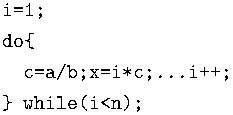
\includegraphics[scale=.7]{ex6_8_1.pdf}
       & $\Rightarrow$ &
      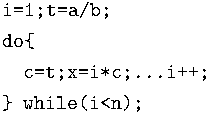
\includegraphics[scale=.7]{ex6_8_2.pdf} \\[1zw]
      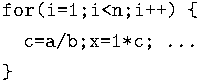
\includegraphics[scale=.7]{ex6_8_3.pdf}
       & $\Rightarrow$ &
      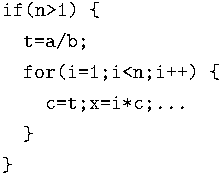
\includegraphics[scale=.7]{ex6_8_4.pdf} \\[1zw]
      \multicolumn{3}{l}{例6.9}                \\
      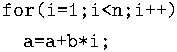
\includegraphics[scale=.7]{ex6_9_1.pdf}
       & $\Rightarrow$ &
      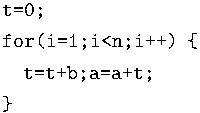
\includegraphics[scale=.7]{ex6_9_2.pdf}
    \end{tabular}
  \end{center}
\end{frame}

\begin{frame}
  \frametitle{ループ最適化(2/3)}
  \begin{list}{}{}
    \item 帰納変数消去\\
          \greentext{帰納変数(ループを制御する変数)は減らす。}\\
          \greentext{参照数の減少}
          \begin{center}
            \begin{tabular}{ccc}
              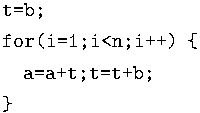
\includegraphics[scale=.75]{ex6_10_1.pdf}
               & $\Rightarrow$ &
              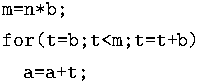
\includegraphics[scale=.75]{ex6_10_2.pdf}
            \end{tabular}
          \end{center}

    \item ループ融合とループ分離\\
    \item ループ展開とソフトウェアパイプライン
  \end{list}
\end{frame}

\begin{frame}
  \frametitle{ループ展開とソフトウェアパイプライン}
  \begin{center}
    \begin{tabular}{ccc}
      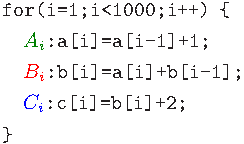
\includegraphics[scale=.75]{ex6_14_1.pdf}
       & $\Rightarrow$ &
      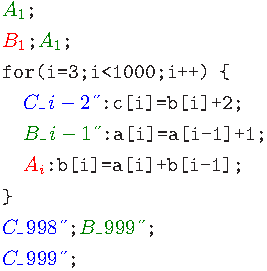
\includegraphics[scale=.75]{ex6_14_2.pdf}
      \\
    \end{tabular}

    \[
      \begin{array}{c|ccc}
               & P_1                        & P_2 & P_3 \\\hline
        1      & A_1                        &     &     \\
        2      & B_1                        & A_2 &     \\
        3      & C_1                        & B_2 & A_3 \\
        4      & A_4                        & C_2 & B_3 \\
        5      & B_4                        & A_5 & C_3 \\
        \vdots & \multicolumn{3}{c}{\vdots}             \\
      \end{array}
    \]
    並列に実行可能
  \end{center}
\end{frame}

\begin{frame}
  \frametitle{手続き呼出し最適化}

  \begin{list}{}{}
    \item {\bf インライン展開}:\ \\
          手続き呼出し=駆動レコードを用いてスタック上に情報を保存

          \greentext{操作としてはコストが大きい}

          スタック操作：実メモリへの正確な順序での書き込みを要求

          短い手続きや関数であればそのまま置き換えてしまった方が
          効率がよい。

    \item {\bf 末尾再帰}:\\

          手続の最後の再帰よびだしは、gotoに置き換え可能。

          \greentext{呼出しから復帰しても駆動レコード上の局所環境を使って
            実行する命令が存在しない。局所領域も再利用可能}
  \end{list}

\end{frame}

\begin{frame}
  \frametitle{末尾再帰の例}
  \begin{tabular}{ccc}
    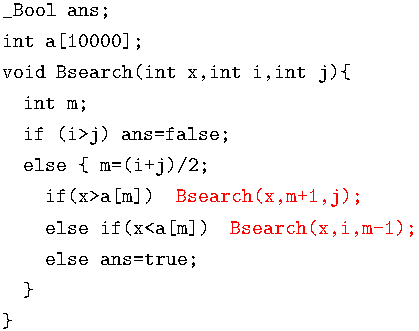
\includegraphics[scale=.6]{ex6_16_1.pdf}
     & $\Rightarrow$ &
    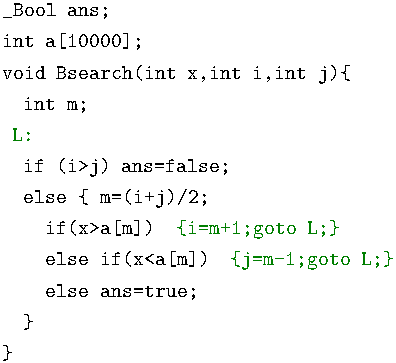
\includegraphics[scale=.6]{ex6_16_2.pdf} \\
     &               & $\Downarrow$          \\
     &               &
    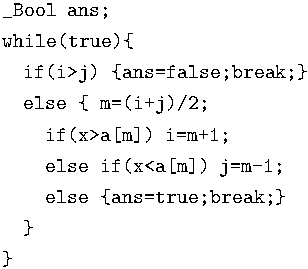
\includegraphics[scale=.6]{ex6_16_3.pdf}
  \end{tabular}
\end{frame}

\subsection{データフロー解析}

\begin{frame}
  \frametitle{データフロー解析}

  \vspace*{10pt}

  \greentext{(講義資料6.4:詳細については省略)}

  \vspace*{10pt}

  基本ブロック$B$に対するデータフロー

  \[
    out[B]=gen[B]\cup(in[B]-kill[B])
  \]

  プログラム上での位置(行番号)：
  \begin{tabular}{ll}
    $in[B]$   & $B$に入力されるデータ  \\
    $out[B]$  & $B$から出力されるデータ \\
    $gen[B]$  & $B$で定義されるデータ  \\
    $kill[B]$ & $B$で上書きされるデータ \\
  \end{tabular}

  入力から出力への制御がきまっていればよいので、基本ブロック単位で考えれ
  ばよい。

  ループ：データフロー方程式を解いて全体的に必要なデータを計算する。
\end{frame}

\begin{frame}{データフロー方程式}
  % \begin{tabular}{ccc}
  %  \begin{minipage}{.2\textwidth}
  % \begin{tikzpicture}
  %  \node[draw] (S1) at (0,1.5) {$S_1$};
  %  \node[draw] (S2) at (0,0) {$S_2$};
  %  \path[->] (S1) edge (S2);
  % \end{tikzpicture}
  %  \end{minipage}
  %  &
  %  \begin{minipage}{.25\textwidth}
  %   \begin{tikzpicture}
  %    
  %   \end{tikzpicture}
  %  \end{minipage}
  % \end{tabular}

  \greentext{定義到達可能性解析：}

  \scalebox{0.7}{
    \begin{tikzpicture}
      \node[draw] (B5) at (2,0) {EXIT};
      \node[draw] (B4) at (2,1.25) {$\begin{array}{ll}d_7: &
             \texttt{i=u3} \\ & \texttt{if...}\end{array}$};
      \node[draw] (B3) at (0,2.25) {$d_6$:\texttt{a=u2}};
      \node[draw] (B2) at (2,3.5) {$\begin{array}{ll}
            d_4: & \texttt{i=i+1}  \\[-3pt]
            d_5: & \texttt{j=j-1}  \\[-3pt]
                 & \texttt{if ...}
          \end{array}$};
      \node[draw] (B1) at (2,5.25) {$\begin{array}{ll}
            d_1: & \texttt{i=m-1} \\[-3pt]
            d_2: & \texttt{j=n}   \\[-3pt]
            d_3: & \texttt{a=u1}
          \end{array}$};
      \node[draw] (B0) at (2,6.75) {ENTRY};

      \node at ($(B1)+(1.75,0)$) {$B_1$};
      \node at ($(B2)+(1.75,0)$) {$B_2$};
      \node at ($(B3)+(1.2,0)$) {$B_3$};
      \node at ($(B4)+(1.75,0)$) {$B_4$};

      \path[->] (B0) edge (B1) (B1) edge (B2) (B2) edge (B4)
      (B2) edge (B3) (B3) edge (B4) (B4) edge (B5);
      \path[->] (B4) [out=210,in=150,looseness=3] edge (B2);

      \node[anchor=west] at ($(B1)+(2.5,0)$) {$\begin{array}{ll}
            gen_{B_1}  & = \{d_1,d_2,d_3\}     \\[-3pt]
            kill_{B_1} & = \{d_4,d_5,d_6,d_7\}
          \end{array}$};
      \node[anchor=west] at ($(B2)+(2.5,0)$) {$\begin{array}{ll}
            gen_{B_2}  & = \{d_4,d_5\}     \\[-3pt]
            kill_{B_2} & = \{d_1,d_2,d_7\}
          \end{array}$};
      \node[anchor=west] at ($(B3)+(4.5,0)$) {$\begin{array}{ll}
            gen_{B_3}  & = \{d_6\} \\[-3pt]
            kill_{B_3} & = \{d_3\}
          \end{array}$};
      \node[anchor=west] at ($(B4)+(2.5,0)$) {$\begin{array}{ll}
            gen_{B_4}  & = \{d_7\}     \\[-3pt]
            kill_{B_4} & = \{d_1,d_4\}
          \end{array}$};
    \end{tikzpicture}
  }

  \vspace*{-30pt}

  {\footnotesize
    \begin{eqnarray*}
      IN[B_2] & = & OUT[B_1]\cup OUT[B_4]\\
      OUT[B_2] & = & gen_{B_2}\cup(IN[B_2]-kill_{B_2})
    \end{eqnarray*}
  }

  (Ahoら：Compilers より引用)
\end{frame}

\begin{frame}
  \frametitle{データフロー方程式}
  \[
    \begin{array}{rcl}
      OUT[B_1] & = & gen_{B_1}                         \\
      IN[B_2]  & = & OUT[B_1]\cup OUT[B_4]             \\
      OUT[B_2] & = & gen_{B_2}\cup(IN[B_2]-kill_{B_2}) \\
      IN[B_3]  & = & OUT[B_2]                          \\
      OUT[B_3] & = & gen_{B_3}\cup(IN[B_3]-kill_{B_3}) \\
      IN[B_4]  & = & OUT[B_3]\cup OUT[B_2]             \\
      OUT[B_4] & = & gen_{B_4}\cup(IN[B_4]-kill_{B_4})
    \end{array}
  \]
\end{frame}

\begin{frame}{データフロー方程式の計算}

  到達可能性解析：

  {\small
  {XXXX XXX}:$d_1,d_2,\cdots,d_7$が集合に入っているとき$1$、入ってないとき$0$
  }

  \vspace*{10pt}

  {\footnotesize
    \begin{tabular}{c|c|c|c|c|c}\hline
      Block $B$ & OUT[$B$]$^0$ & IN[$B$]$^1$ & OUT[$B$]$^1$ & IN[$B$]$^2$ & OUT[$B$]$^2$ \\\hline
      $B_1$     & 111 0000     & 000 0000    & 111 0000     & 000 0000    & 111 0000     \\
      $B_2$     & 000 1100     & 111 0001    & 001 1100     & 111 0111    & 001 1110     \\
      $B_3$     & 000 0010     & 000 1100    & 000 1110     & 001 1100    & 000 1110     \\
      $B_4$     & 000 0001     & 000 1110    & 000 0111     & 001 1110    & 001 0111     \\\hline
    \end{tabular}
  }

  \vspace*{10pt}

  \greentext{変化しなくなるまでくりかえす。}


  $OUT[B_4]$=001 0111:\\
  \greentext{本ブロックでは$d_3$,$d_5$,$d_6$,$d_7$がEXITが到達する可能性がある．}

\end{frame}

\begin{frame}
  \frametitle{データフロー}
  \greentext{生存解析}
  \begin{tabular}{ll}
    $Use[B]$: & $B$で再定義される前に資料される変数の集合 \\
    $Def[B]$: & $B$で定義される変数の集合
  \end{tabular}

  \begin{eqnarray*}
    In[B] & = & Use[B]\cup(Out[B]-Def[B])\\
    Out[B] & = & \cup_{S\in Succ[B]}In[S]
  \end{eqnarray*}
  $Succ[B]$: フローグラフにおいて$B$から直接フローがあるブロック
\end{frame}

\begin{frame}
  \frametitle{データフロー解析}
  \scalebox{0.7}{
    \begin{tikzpicture}
      \node[draw] (B5) at (2,0) {EXIT};
      \node[draw] (B4) at (2,1.25) {$\begin{array}{ll}d_7: &
             \texttt{i=u3} \\ & \texttt{if...}\end{array}$};
      \node[draw] (B3) at (0,2.25) {$d_6$:\texttt{a=u2}};
      \node[draw] (B2) at (2,3.5) {$\begin{array}{ll}
            d_4: & \texttt{i=i+1}  \\[-3pt]
            d_5: & \texttt{j=j-1}  \\[-3pt]
                 & \texttt{if ...}
          \end{array}$};
      \node[draw] (B1) at (2,5.25) {$\begin{array}{ll}
            d_1: & \texttt{i=m-1} \\[-3pt]
            d_2: & \texttt{j=n}   \\[-3pt]
            d_3: & \texttt{a=u1}
          \end{array}$};
      \node[draw] (B0) at (2,6.75) {ENTRY};

      \node at ($(B1)+(1.75,0)$) {$B_1$};
      \node at ($(B2)+(1.75,0)$) {$B_2$};
      \node at ($(B3)+(1.2,0)$) {$B_3$};
      \node at ($(B4)+(1.75,0)$) {$B_4$};

      \path[->] (B0) edge (B1) (B1) edge (B2) (B2) edge (B4)
      (B2) edge (B3) (B3) edge (B4) (B4) edge (B5);
      \path[->] (B4) [out=210,in=150,looseness=3] edge (B2);

      \node[anchor=west] at ($(B1)+(2.5,0)$) {$\begin{array}{ll}
            Def_{B_1} & = \{i,j,a\}   \\[-3pt]
            Use_{B_1} & = \{m,n,u_1\}
          \end{array}$};
      \node[anchor=west] at ($(B2)+(2.5,0)$) {$\begin{array}{ll}
            Def_{B_2} & = \{i,j\} \\[-3pt]
            Use_{B_2} & = \{i,j\}
          \end{array}$};
      \node[anchor=west] at ($(B3)+(4.5,0)$) {$\begin{array}{ll}
            Def_{B_3} & = \{a\}  \\[-3pt]
            Use_{B_3} & = \{u2\}
          \end{array}$};
      \node[anchor=west] at ($(B4)+(2.5,0)$) {$\begin{array}{ll}
            Def_{B_4} & = \{i\}  \\[-3pt]
            Use_{B_4} & = \{u3\}
          \end{array}$};
    \end{tikzpicture}
  }
\end{frame}

\begin{frame}
  \frametitle{データフロー解析（生存解析）}
  $(a,i,j,m,n,u1,u2,u3)$とすると

  {\scriptsize
  $\begin{array}{l|llllll}
          & OUT        & IN         & OUT        & IN         & OUT        & IN         \\\hline
      B_1 & (00000000) & (00011100) & (01100000) & (00011100) & (01100010) & (00011100) \\
      B_2 & (00000000) & (01100000) & (01100010) & (01100010) & (01100001) & (01100010) \\
      B_3 & (00000000) & (00000010) & (00000001) & (00000010) & (00100001) & (10100001) \\
      B_4 & (00000000) & (00000001) & (01100000) & (00100001) & (01100010) & (00100001)
    \end{array}$}

  \vspace*{10pt}

  \greentext{\small フローグラフの基本ブロックにおいてどの変数が影響をうけるかを解析}

  \vspace*{10pt}

  $\begin{array}{l|ll}
          & IN         & OUT        \\\hline
      B_1 & \{m,n,u1\} & \{i,j,u2\} \\
      B_2 & \{i,j,u2\} & \{i,j,u3\} \\
      B_3 & \{a,j,u3\} & \{j,u3\}   \\
      B_4 & \{j,u3\}   & \{i,j,u2\}
    \end{array}$
\end{frame}

% \begin{frame}[fragile]
%  \frametitle{配列参照}

% \begin{enumerate}
%  \item $\mathtt{x = a[i]}$の形の配列参照\\
%        演算子\texttt{=[]}のノードを生成し、子として$a_0$および$i$、
%        ノードに$x$をラベルづけする。
%  \item \texttt{a[i]=x}の形の配列代入\\
%        演算子\texttt{[]=]}のノードを生成し、
%        子として、$a_0$, $i$, $x$をとり、$a_0$を参照している
%        \texttt{=[]}ノードに'killed'マークをつける。
%        $a[i]$は共通部分式として用いることはできない。
% \end{enumerate}

%  \vspace*{0.5cm}

%  \begin{tabular}{ccc}
%  \begin{tabular}{l}
% {\tt x = a[i]}\\
% {\tt a[j]=y}\\
% {\tt z=a[i]}
%  \end{tabular}
%   & \hspace*{1cm} &

% \begin{tikzpicture}
%  \node (a0) at (0,0) {$a_0$};
%  \node (i0) at (1.5,0) {$i_0$};
%  \node (j0) at (3,0) {$j_0$};
%  \node (y0) at (4.5,0) {$y_0$};

%  \node[draw] (Ar1) at (0.75,1) {\texttt{=[]}};
%  \node[draw] (Ar2) at (3.75,1) {\texttt{=[]}};

%  \node[draw] (Ar3) at (0.75,2.5) {\texttt{=[]}};

%  \node (Ann0) at (0.75,1.5) {\sf Killed};

%  \node at ($(Ar1)+(0.8,0)$) {$x$};
%  \node at ($(Ar3)+(0.8,0)$) {$z$};

%  \path (a0) edge (Ar2)  (i0) edge (Ar2)  (j0) edge (Ar2) (y0) edge (Ar2);
%  \path (a0) edge (Ar1)  (i0) edge (Ar1);
%  \path (a0) [out=120,in=225] edge (Ar3);
%  \path (i0) [out=60, in=315] edge (Ar3);
% \end{tikzpicture}
%  \end{tabular}

% \end{frame}

% \subsection{大域的最適化}

%  \begin{frame}
%  \frametitle{大域的コード最適化}
%  基本ブロックを越える最適化

%  \begin{list}{}{}
%   \item ループ最適化
%   \item 手続き呼び出し最適化
%   \item データフロー解析
%   \item 静的単一代入(SSA)解析
%  \end{list}
% \end{frame}

% \begin{frame}
%  \frametitle{ループ最適化(1/3)}
%  ループ内のコード実行回数:ループ外のコードよりも一般に多い\\
%  ループ内のコードは慎重に最適化\\
%  本当に毎回実行しなければならないか？できるだけ効率よく実行
%  \begin{list}{}{}
%   \item ループ不変式の移動\\
% 	\greentext{ループから影響をうけない式を外に出す}l\\
% 	例6.8
%   \item ループ内の演算の強さの軽減\\
% 	強い演算：時間のコストが大きい演算\\
% 	足し算$<$掛け算 (加算器$<$乗算器)\\
% 	例6.9
%  \end{list}
% \end{frame}

% \begin{frame}
%  \frametitle{例}
%  \begin{center}
%  \begin{tabular}{ccc}
%   \multicolumn{3}{l}{例6.8}\\
%   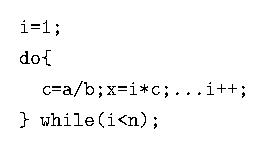
\includegraphics[scale=.7]{ex6_8_1.eps}
%   & $\Rightarrow$ & 
%   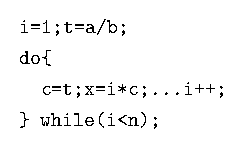
\includegraphics[scale=.7]{ex6_8_2.eps} \\[1zw]
%   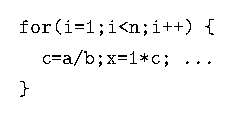
\includegraphics[scale=.7]{ex6_8_3.eps}
%   & $\Rightarrow$ & 
%   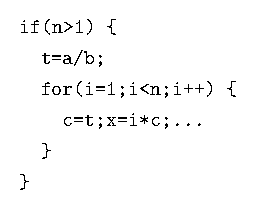
\includegraphics[scale=.7]{ex6_8_4.eps} \\[1zw]
%   \multicolumn{3}{l}{例6.9}\\
%   
\includegraphics[scale=.7]{ex6_9_1.eps}
%   & $\Rightarrow$ & 
%   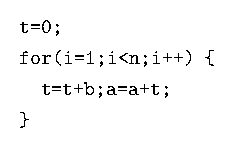
\includegraphics[scale=.7]{ex6_9_2.eps}
%  \end{tabular}
%  \end{center}
% \end{frame}

% \begin{frame}
%  \frametitle{ループ最適化(2/3)}
%  \begin{list}{}{}
%   \item 帰納変数消去\\
% 	\greentext{帰納変数(ループを制御する変数)は減らす。}\\
% 	\greentext{参照数の減少}
% 	\begin{center}
% 	 \begin{tabular}{ccc}
% 	  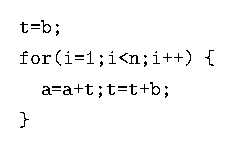
\includegraphics[scale=.75]{ex6_10_1.eps}
% 	  & $\Rightarrow$ &
% 	  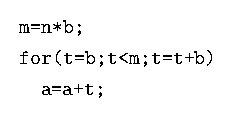
\includegraphics[scale=.75]{ex6_10_2.eps}
% 	 \end{tabular}
% 	\end{center}

%   \item ループ融合とループ分離\\
%   \item ループ展開とソフトウェアパイプライン
%  \end{list}
% \end{frame}

% \begin{frame}
%  \frametitle{ループ展開とソフトウェアパイプライン}
%  \begin{center}
%  \begin{tabular}{ccc}
%   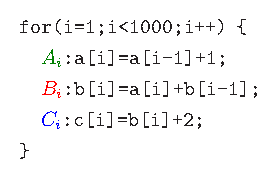
\includegraphics[scale=.75]{ex6_14_1.eps}
%   & $\Rightarrow$ &
%   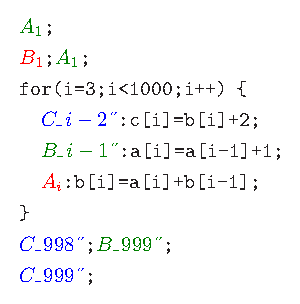
\includegraphics[scale=.75]{ex6_14_2.eps}
%  \\
%  \end{tabular}

%   \[
%    \begin{array}{c|ccc}
%     &P_1 &P_2 &P_3 \\\hline
%    1 & A_1 & & \\
%    2 & B_1 & A_2 & \\
%    3 & C_1 & B_2 & A_3 \\
%    4 & A_4 & C_2 & B_3 \\
%    5 & B_4 & A_5 & C_3 \\
%    \vdots & \multicolumn{3}{c}{\vdots}\\
%    \end{array}
%   \]
%  並列に実行可能
%  \end{center}
% \end{frame}

% \begin{frame}
%  \frametitle{手続き呼出し最適化}

%  \begin{list}{}{}
%   \item {\bf インライン展開}:\ \\
%  手続き呼出し=駆動レコードを用いてスタック上に情報を保存

%  \greentext{操作としてはコストが大きい}

%  スタック操作：実メモリへの正確な順序での書き込みを要求

%  短い手続きや関数であればそのまま置き換えてしまった方が
%  効率がよい。

%   \item {\bf 末尾再帰}:\\

% 	手続の最後の再帰よびだしは、gotoに置き換え可能。

% 	\greentext{呼出しから復帰しても駆動レコード上の局所環境を使って
% 	実行する命令が存在しない。局所領域も再利用可能}
%  \end{list}

% \end{frame}

% \begin{frame}
%  \frametitle{末尾再帰の例}
%  \begin{tabular}{ccc}
%   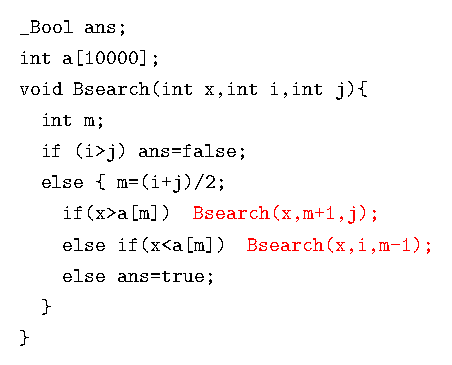
\includegraphics[scale=.6]{ex6_16_1.eps}
%   & $\Rightarrow$ &
%   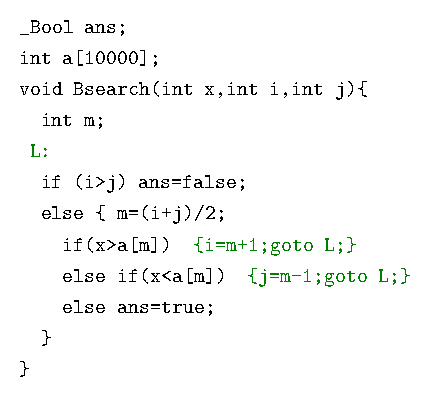
\includegraphics[scale=.6]{ex6_16_2.eps}\\
%   & & $\Downarrow$\\
%   & &
%   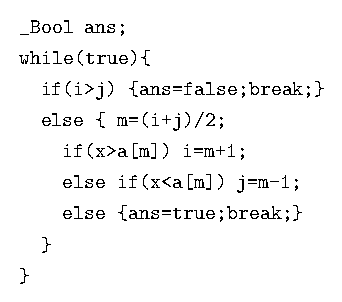
\includegraphics[scale=.6]{ex6_16_3.eps}
%  \end{tabular}
% \end{frame}

% \subsection{データフロー解析}

% \begin{frame}
%  \frametitle{データフロー解析}

%  \vspace*{10pt}

%  \greentext{(教科書6.4:詳細については省略)}

%  \vspace*{10pt}

%  ステートメント$S$に対するデータフロー

%  \[
%   out[S]=gen[S]\cup(in[S]-kill[S])
%  \]

%  プログラム上での位置(行番号)：
%  \begin{tabular}{ll}
%   $in[S]$ & $S$に入力されるデータ\\
%   $out[S]$ & $S$から出力されるデータ\\
%   $gen[S]$ & $S$で定義されるデータ\\
%   $kill[S]$ & $S$で上書きされるデータ\\
%  \end{tabular}

%  入力から出力への制御がきまっていればよいので、基本ブロック単位で考えれ
%  ばよい。

%  ループ：データフロー方程式を解いて全体的に必要なデータを計算する。
% \end{frame}

% \begin{frame}{データフロー方程式}
% % \begin{tabular}{ccc}
% %  \begin{minipage}{.2\textwidth}
% % \begin{tikzpicture}
% %  \node[draw] (S1) at (0,1.5) {$S_1$};
% %  \node[draw] (S2) at (0,0) {$S_2$};
% %  \path[->] (S1) edge (S2);
% % \end{tikzpicture}
% %  \end{minipage}
% %  &
% %  \begin{minipage}{.25\textwidth}
% %   \begin{tikzpicture}
% %    
% %   \end{tikzpicture}
% %  \end{minipage}
% % \end{tabular}

% \scalebox{0.7}{
% \begin{tikzpicture}
%  \node[draw] (B5) at (2,0) {EXIT};
%  \node[draw] (B4) at (2,1) {$d_7$:\texttt{i=u3}};
%  \node[draw] (B3) at (0,2) {$d_6$:\texttt{a=u2}};
%  \node[draw] (B2) at (2,3.25) {$\begin{array}{ll}
%   d_4: & \texttt{i=i+1}\\[-3pt]
%   d_5: & \texttt{j=j-1}
% 		       \end{array}$};
%  \node[draw] (B1) at (2,5) {$\begin{array}{ll}
%   d_1: & \texttt{i=m-1}\\[-3pt]
%   d_2: & \texttt{j=n}\\[-3pt]
%   d_3: & \texttt{a=u1}
% 			\end{array}$};
%  \node[draw] (B0) at (2,6.5) {ENTRY};

%  \node at ($(B1)+(1.5,0)$) {$B_1$};
%  \node at ($(B2)+(1.5,0)$) {$B_2$};
%  \node at ($(B3)+(1.2,0)$) {$B_3$};
%  \node at ($(B4)+(1.2,0)$) {$B_4$};

%  \path[->] (B0) edge (B1) (B1) edge (B2) (B2) edge (B4)
%            (B2) edge (B3) (B3) edge (B4) (B4) edge (B5);
%  \path[->] (B4) [out=210,in=150,looseness=3] edge (B2);

%  \node[anchor=west] at ($(B1)+(2.5,0)$) {$\begin{array}{ll}
%   gen_{B_1} & = \{d_1,d_2,d_3\}\\[-3pt]
%   kill_{B_1} & = \{d_4,d_5,d_6,d_7\}
% 			   \end{array}$};
%  \node[anchor=west] at ($(B2)+(2.5,0)$) {$\begin{array}{ll}
%   gen_{B_2} & = \{d_4,d_5\} \\[-3pt]
%   kill_{B_2} & = \{d_1,d_2,d_7\}
% 			   \end{array}$};
%  \node[anchor=west] at ($(B3)+(4.5,0)$) {$\begin{array}{ll}
%   gen_{B_3} & = \{d_6\}\\[-3pt]
%   kill_{B_3} & = \{d_3\}
% 			   \end{array}$};
%  \node[anchor=west] at ($(B4)+(2.5,0)$) {$\begin{array}{ll}
%   gen_{B_4} & = \{d_7\} \\[-3pt]
%   kill_{B_4} & = \{d_1,d_4\}
% 			   \end{array}$};

% \end{tikzpicture}
% }

% {\footnotesize
% \begin{eqnarray*}
%  IN[B_2] & = & OUT[B_1]\cup OUT[B_4]\\
%  OUT[B_2] & = & gen_{B_2}\cup(IN[B_2]-kill_{B_2})
% \end{eqnarray*}
% }

% (Ahoら：Compilers より引用)
% \end{frame}

% \begin{frame}{データフロー方程式の計算}

% 到達可能性解析：

% {\small
% {XXXX XXX}:$d_1,d_2,\cdots,d_7$が集合に入っているとき$1$、入ってないとき$0$
% }

% \vspace*{10pt}

% {\footnotesize
% \begin{tabular}{c|c|c|c|c|c}\hline
% Block $B$ & OUT[$B$]$^0$ & IN[$B$]$^1$ & OUT[$B$]$^1$ & IN[$B$]$^2$ & OUT[$B$]$^2$\\\hline
% $B_1$ & 000 0000 & 000 0000 & 111 0000 & 000 0000 & 111 0000\\
% $B_2$ & 000 0000 & 111 0000 & 001 1100 & 111 0111 & 001 1110\\
% $B_3$ & 000 0000 & 001 1100 & 000 1110 & 001 1110 & 000 1110\\
% $B_4$ & 000 0000 & 001 1110 & 001 0111 & 001 1110 & 001 0111\\
% EXIT  & 000 0000 & 001 0111 & 001 0111 & 001 0111 & 001 0111\\\hline
% \end{tabular}
% }

% \vspace*{10pt}

% \greentext{変化しなくなるまでくりかえす。}


% OUT[EXIT]=001 0111:\\
% \greentext{本ブロックでは$d_3$,$d_5$,$d_6$,$d_7$がEXITが到達する}

% \end{frame}


\end{document}
